\documentclass[11pt]{article}
\usepackage{amsmath,amssymb,xspace,epsfig}
\usepackage{algorithm}
\usepackage{algpseudocode}
\usepackage{algorithmicx}
\usepackage{graphicx}
\usepackage{subfigure}

\graphicspath{{plots/}}


\textwidth 6.5in \textheight 9.05in \oddsidemargin 0.0in
\evensidemargin 0.0in \topmargin -0.55in
\addtolength{\textwidth}{2.5mm} \addtolength{\columnsep}{2mm}

\title{Report of assignment 1}
\author{Haoyang Zhang, Qi Wu, Shengjie Li}


\begin{document}
\maketitle

	\section*{Questions}
	\begin{enumerate}
		\item what do you expect to happen if an IF neuron is constantly fed a very low input current? An LIF neuron?
		
		IF: See Figure \ref{fig:Fig1.sub.L}. Because the neuron continually integrates input, its membrane potential $V_m$ will constantly grow up. Finally, $V_m$ will reach the threshold $V_{threshold}$. Then, the neuron will fire and reset $V_m$.
		
		LIF: See Figure\ref{fig:Fig1.sub.L}. At the beginning, because the input current $I$ is far smaller than $-V_m/R_m$, voltage is dominated by "leak", the voltage will increase steeply from $V_{rest}$. Then, as voltage $V_m$ increasing, $-V_m/R_m$ will decrease and be close or equal to the input current $I$. So, $dV/dt$ will be close to 0. Because the input can not exceed the threshold $V_m/R_m$, it will be leaked out. Therefore, finally the voltage will converge to $R_mI$, where $dV/dt = 0$. Also, because $I < V_{threshold}/R_m$, this neuron will never fire.
		
		\item what do you expect to happen if an IF neuron is constantly fed a large input current? An LIF neuron?
			
		IF: See Figure \ref{fig:Fig1.sub.H}\ref{fig:Fig1.sub.I}. Because the input current is large, the ?gradient? of voltage is also large. Therefore, neuron will fire and reset in a very high frequency.
		
		LIF: See Figure \ref{fig:Fig1.sub.H}\ref{fig:Fig1.sub.I}. Because the input current $I$ is very large, the current "leak" can not counteract the input. Therefore, the membrane potential is dominated by input current, and the neuron has a similar performance as IF. However, LIF model still fire in a higher frequency than IF model. This is because the "leak term" $V_m/R_m$ accelerates the increasing of voltage when the voltage is negative.
		
		\item What are the limitations of an LIF neuron?
			
		The LIF neuron can't handle large input. See \ref{fig:Fig1.sub.I}, when input current is large, the "leak term" of LIF model lost its function, and LIF will have a similar performance as IF. ?all spikes are the same?
		
			\begin{figure}[htb]
			\centering
			\subfigure[Low input]{
			\label{fig:Fig1.sub.L}
			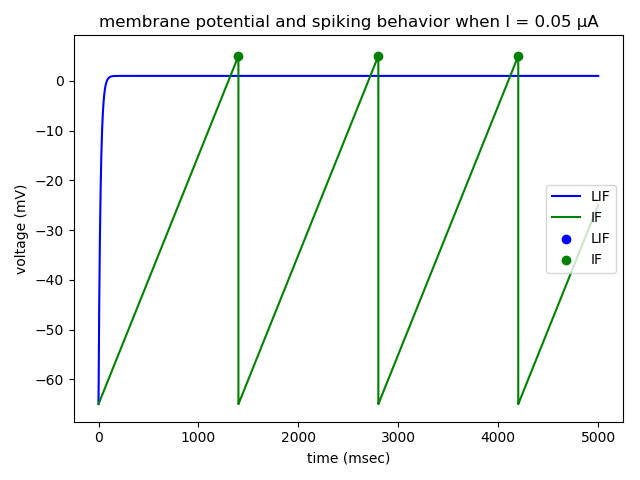
\includegraphics[scale=0.2]{plot_question_1.png}}
			\subfigure[High input]{
			\label{fig:Fig1.sub.H}
			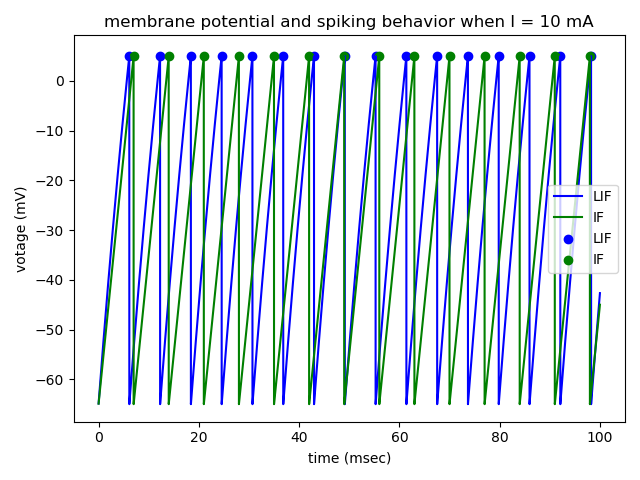
\includegraphics[scale=0.2]{plot_question_2.png}}
			\subfigure[Increasing input]{
			\label{fig:Fig1.sub.I}
			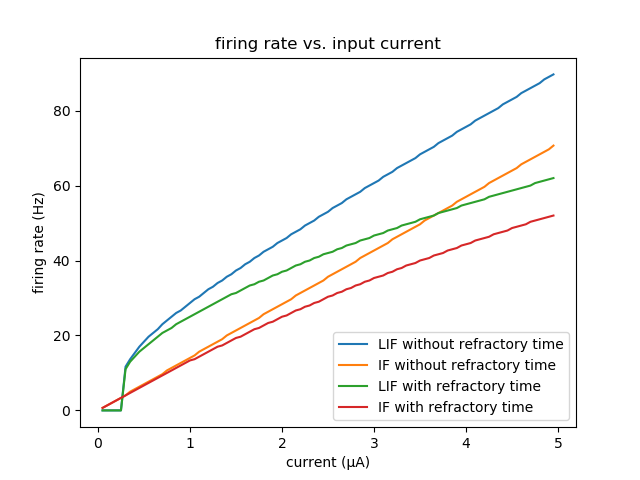
\includegraphics[scale=0.2]{plot_question_3.png}}
			\caption{LIF and IF}
			\end{figure}
		
	\end{enumerate}
	
	\section*{Programing}
	\begin{enumerate}
		\item Simulate an LIF neuron with different input currents and plot the membrane potential, showing (a) potential decay over time and (b) spiking behavior.

		See \ref{fig:Fig2.sub.voltage}. The typical value we use is $V_{rest} = -65$, $V_{threshold} = 5$, $C_m = 1$, and $R_m = 20$.
		
		\item Plot the firing rate as a function of the input current.
		
		See \ref{fig:Fig2.sub.voltage}.
		
		\begin{figure}[htb]
			\centering
			\subfigure[Potential]{
			\label{fig:Fig2.sub.voltage}
			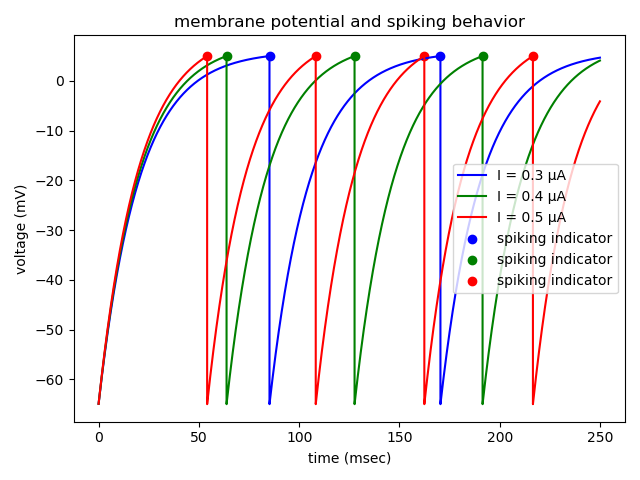
\includegraphics[scale=0.3]{plot_programming_1.png}}
			\subfigure[Firing rate]{
			\label{fig:Fig2.sub.fire_rate}
			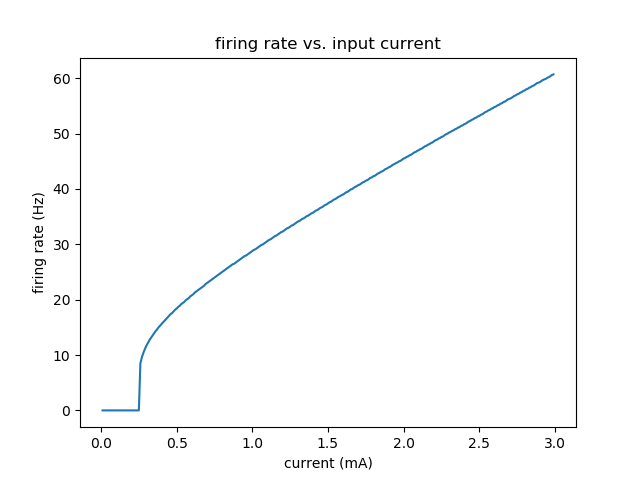
\includegraphics[scale=0.3]{plot_programming_2.png}}
			\caption{LIF and IF}
		\end{figure}
		
		\item What happens to the firing rate as you continue to increase the input current? Why?
		
		See \ref{fig:Fig2.sub.fire_rate}. When the input current is very small $I < V_{threshold}/R_m$, the neuron doesn't fire. Then, as the current increasing, the firing rate will increase steeply. This is because ?. As input current increasing, because the potential will be reseted to $V_{rest}$ after firing, $R_mI$ will be far larger than $V$. In this case, the potential will be dominated by input current, and the firing rate will be linear correlation with input current.
		
		\item Simulate a neuron using the Izhikevich model.
		
		See \ref{fig:Fig4.sub.Izh}. The typical value is that $a = 0.02$, $b - 0.2$, $c - -65$, $d = 8$, and $V_{threshold} = 30$.
		
		\item Simulate a neuron using the Hodgkin-Huxley model.
		
		See \ref{fig:Fig4.sub.H-H}. The typical value is that $\bar{g_k} = 36$, $\bar{g_{na}} = 120$, $\bar{g_l} = 0.3$, $V_k = -12$, $V_{na} = 115$, $V_l = 10.6$.
		
		\begin{figure}[htb]
			\centering
			\subfigure[Izhikevich]{
			\label{fig:Fig4.sub.Izh}
			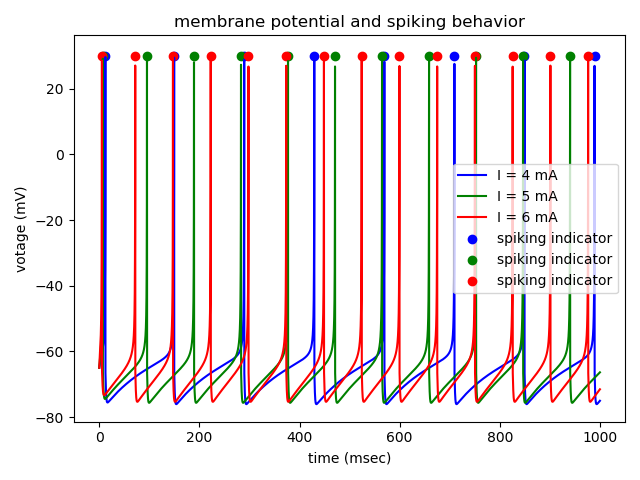
\includegraphics[scale=0.3]{plot_programming_4.png}}
			\subfigure[Hodgkin-Huxley]{
			\label{fig:Fig4.sub.H-H}
			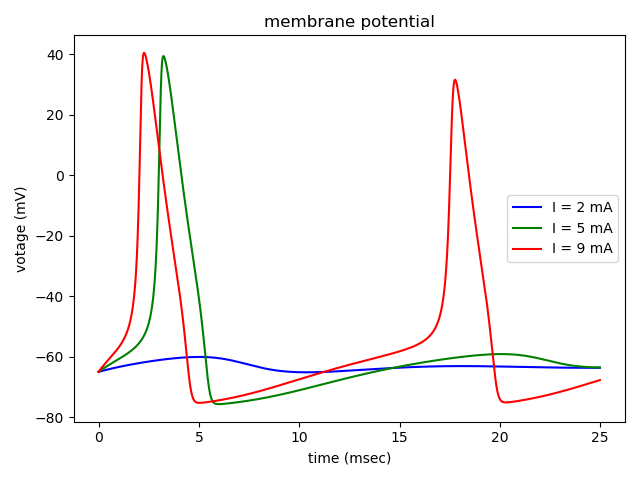
\includegraphics[scale=0.3]{plot_programming_5.png}}
			\caption{Izhikevich and Hodgkin-Huxley}
		\end{figure}
		
		\item Assume that you administer a drug named TTX, which inhibits the sodium current. Simulate the effect that TTX would have on the neural firing. Do the same for another drug, pronase, which eliminated sodium inactivation.
		
		TTX:
		
		Because TTX will inhibit the sodium current, sodium particle can not enter or exit the neuron. This situation is equal to closing all the sodium channel. Therefore, we can set 0 for $g_{na}m^3h(V-V_na)$ to simulate the effect of TTX. See the green curve in \ref{fig:fig5}.
		
		Pronase:
		
		Pronase will eliminate the sodium inactivation. Therefore, all inactivation gate will keep open. So, we can fixed $h$ to 1 to simulate this effect. See the red curve in \ref{fig:fig5}.
		
		\begin{figure}[htb]
			\centering
			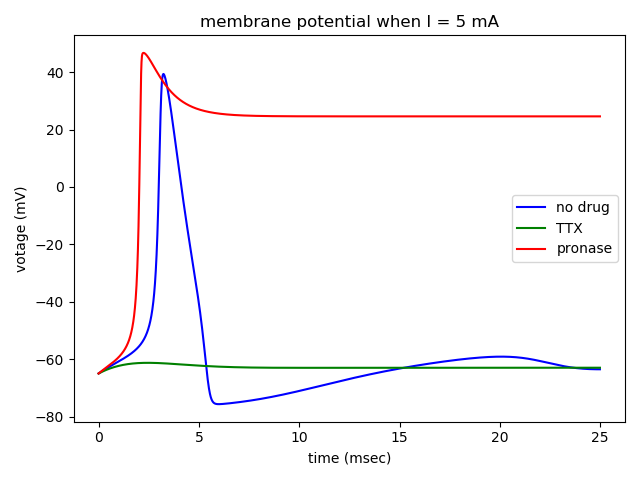
\includegraphics[scale=0.3]{plot_programming_7.png}
			\caption{TTX and pronase}
			\label{fig:fig5}
		\end{figure}
	\end{enumerate}
\end{document}